%------------------------------------------------------------
\chapter{流体方程式の数値解法}
%------------------------------------------------------------

%
%\begin{equation}
%    \frac{\partial \bm{ U}}{\partial t} 
%    + \frac{\partial \bm{ F}}{\partial x}
%    + \frac{\partial \bm{ G}}{\partial y}
%    + \frac{\partial \bm{ H}}{\partial z}=0
%\end{equation}
%\begin{equation}
%    \bm{ U} = \left( 
%        \begin{array}{c}
%            \rho \\
%            \rho v_x \\
%            \rho v_y \\
%            \rho v_z \\
%            E
%    \end{array}
%\right),\;\;
%    \bm{ F} = \left( 
%        \begin{array}{c}
%            \rho v_x \\
%            \rho v_x^2 + P \\
%            \rho v_x v_y \\
%            \rho v_x v_z \\
%            (E + P)v_x
%    \end{array}
%\right),\;\;
%    \bm{ G} = \left( 
%        \begin{array}{c}
%            \rho v_y \\
%            \rho v_y v_x \\
%            \rho v_y^2 + P \\
%            \rho v_y v_z \\
%            (E + P)v_y
%    \end{array}
%\right),\;\;
%    \bm{ G} = \left( 
%        \begin{array}{c}
%            \rho v_z \\
%            \rho v_z v_x \\
%            \rho v_z v_y \\
%            \rho v_z^2 + P  \\
%            (E + P)v_z
%    \end{array}
%\right),\;\;
%\end{equation}
%%%%
%
%%----------------------------------------------------------------------
%\newpage
%\section{一次元数値流体計算法}
%%----------------------------------------------------------------------
この章では、以下の1次元流体方程式の数値解法について扱う。
高精度化と多次元化については次の磁気流体方程式の数値解法の章(第\ref{chap:mhd}章)で説明する。
\begin{equation}
    \frac{\partial \bm{ U}}{\partial t} 
    + \frac{\partial \bm{ F}}{\partial x}=0
\end{equation}
\begin{equation}
    \bm{ U} = \left( 
        \begin{array}{c}
            \rho \\
            \rho v_x \\
            E
    \end{array}
\right),\;\;
    \bm{ F} = \left( 
        \begin{array}{c}
            \rho v_x \\
            \rho v_x^2 + P \\
            (E + P)v_x
    \end{array}
\right)
\label{hydro1d_eq}
\end{equation}

流体方程式の数値解法については様々な手法が提案されてきた。
CfCA流体学校では、
現在の天文シミュレーションにおいて広く用いられているGodunov法
\citep{Godunov1959}とそこから派生した手法を主に扱う。
その前に、移流方程式の数値解法で開発された手法の流体方程式への
応用についても、Riemann不変量や特性曲線などの重要事項が出てくる
とともに歴史的に重要なので簡単に説明する。

%---------------------------------------
\section{移流方程式の数値解法の流体方程式への適用}\label{sec:advection}
%---------------------------------------

%------------------------------
\subsection{移流方程式の数値解法}
%------------------------------
最も簡単な双曲型微分方程式である移流方程式
\begin{equation}
    \frac{\partial u}{\partial t} + c\frac{\partial u}{\partial x}=0
    \label{advection}
\end{equation}
は、物理量$f$の速度$c$での移流を表しており、
厳密解$u=f(x-ct)$が知られている。

移流方程式の数値解法については長い歴史があり、移流方程式の発展形である流体方程式の数値解法に


\begin{equation}
u_i^{n+1} = u_i^n - \nu (f_{i+1/2} - f_{i-1/2}),
\end{equation}
ここで、$\nu = c \Delta t/\Delta x$。

数値流束$f_{i+1/2}$の様々な評価方法がある。
詳細な解説は講義に譲り、ここでは代表的なものについて列挙する。

\noindent
\underline{\bf 中心差分}

差分方程式は、
\begin{equation}
    u_i^{n+1} = u^n - \nu \frac{1}{2} \left( u_{i+1} - u_{i-1}\right)
\end{equation}
となり、有限体積法での数値流束は
\begin{equation}
    f_{i+1/2} = 
    c \frac{u_i+u_{i+1}}{2}
\end{equation}
となる。中心差分は数値的に不安定である。

\noindent
\underline{\bf 空間一次精度風上差分}

差分方程式は、$c$の正負により後退差分と前進差分を切り替えて、
\begin{equation}
    u_i^{n+1} = 
    \left\{
    \begin{array}{ll}
    u^n - \nu \left( u_{i} - u_{i-1}\right) & \mathrm{for}\;\; c>0 \\
    u^n - \nu \left( u_{i+1} - u_{i}\right) & \mathrm{for}\;\; c<0
    \end{array}
    \right.
\end{equation}
となり、数値流束は
\begin{equation}
    f_{i+1/2} = 
    \left\{
    \begin{array}{ll}
         c u_i & \mathrm{for}~ c> 0 \\
         c u_{i+1} & \mathrm{for}~ c<0 \\
    \end{array}
    \right.
\end{equation}
となる。また以下のようにまとめて書くこともできる。
\begin{equation}
    f_{i+1/2} = 
    \left\{
    \frac{cu_i+cu_{i+1}}{2}
     - \frac{|c|}{2}(u_{i+1} - u_i) 
    \right\}
\end{equation}

\noindent
\underline{\bf Lax法}

差分方程式\citep{Lax1954}は、
\begin{equation}
    u_i^{n+1} = \frac{u_{i-1}^n + u_{i+1}^n}{2} - \frac{\nu}{2} \left( u_{i+1} - u_{i-1}\right)
\end{equation}
となり、数値流束は、
\begin{equation}
    f_{i+1/2} = 
    c\left(
    \frac{1+1/\nu}{2} u_{i}
    + \frac{1-1/\nu}{2} u_{i+1}
    \right)
    = 
    c\left(
    \frac{u_i+u_{i+1}}{2}
    \right)
     - \frac{\Delta x}{2\Delta t}(u_{i+1} - u_i) 
\end{equation}
となる。

\noindent
\underline{\bf Lax-Wendroff法}

差分方程式\citep{LaxWendroff1960}は、
\begin{equation}
    u_i^{n+1} = u_i^n 
    - \frac{\nu}{2} \left( u_{i+1} - u_{i-1}\right)
    + \frac{\nu^2}{2} \left( u_{i+1} - 2u_i + u_{i-1}\right)
\end{equation}
となり、数値流束は、
\begin{equation}
    f_{i+1/2} = 
    c\left(
    \frac{1+\nu}{2} u_{i}
    + \frac{1-\nu}{2} u_{i+1}
    \right)
    = 
    c\left\{
    \frac{u_i+u_{i+1}}{2}
     - \frac{\nu}{2}(u_{i+1} - u_i) 
    \right\}
\end{equation}
となる。

Lax法とLax-Wendroff法は、セル境界$i+1/2$の両側のセル中心の値
$u_i$と$u_{i+1}$をある重みを付けて平均した値で流束を
評価していることになっている。
また、別の見方をすると、
数値流束は中心差分での数値流束に、$u_{i+1}-u_i$に比例する
項を加えた形に変形することができる。
$u_{i+1}-u_i \sim (\partial u/\partial x)\Delta x$
なので、拡散として働き、
その拡散係数はLax法では$c\Delta x/\nu=\Delta x^2/\Delta t$、Lax-Wendroff法では
$\nu c\Delta x=c^2\Delta t $となる。
数値的に不安定な中心差分を拡散で安定化していると解釈することができる。
ただその大きさは両者で異なり、Lax法は離散化した時空($\Delta x, \Delta t$)で決まる最大の拡散になっており、
Lax-Wendroff法は、移流速度と$\Delta t$の間での移流距離で決まる拡散になっている。
CFL条件より$\nu\le 1$なので、Lax法の方がLax-Wendroff法よりも数値拡散がかなり大きく入る。





%------------------------------
\subsection{特性曲線}
%------------------------------

流体方程式の性質として、


流体方程式はJacobi行列$A$を使うと、以下のように移流方程式に似せた形に書き換えることができる。
\begin{equation}
    \frac{\partial U_i}{\partial t} 
    + A_{ij} \frac{\partial U_j}{\partial x}=0,\;\;\;A_{ij} = \frac{\partial F_i}{\partial U_j}
\end{equation}
\begin{equation}
    A_{ij} = \left( 
        \begin{array}{ccc}
         0  & 1 & 0 \\
       \displaystyle - (3-\gamma)v^2/2  & (3-\gamma) v & \gamma - 1 \\ 
       \displaystyle  
       \left(\frac{(\gamma-2)v^2}{2} - 
       \frac{\gamma P}{\gamma-1} \right)v & 
       \displaystyle \frac{\gamma P}{\gamma-1} +
       \frac{(3-2\gamma)v^2}{2} & \gamma v\\
        \end{array}
    \right)
\end{equation}
$A_{ij}$が移流方程式での速度に対応するが、非対角成分が存在するので、
完全な移流方程式ではない。
そこで$A_{ij}$が対角成分となるような系を変換する。

Jacobi行列の固有値と固有ベクトルは、それぞれ
\begin{equation}
    \lambda_1 = v - a, \lambda_2 = v, \lambda_3 = v+a 
\end{equation}
\begin{equation}
\bm{ r}_1 = 
\left(
        \begin{array}{ccc}
         1  \\
         v-a \\
         H - va \\
        \end{array}
\right),\;\;\;
\bm{ r}_2 = 
\left(
        \begin{array}{ccc}
         1  \\
         v \\
         v^2/2 \\
        \end{array}
\right),\;\;\;
\bm{ r}_3 = 
\left(
        \begin{array}{ccc}
         1  \\
         v+a \\
         H + va \\
        \end{array}
\right),\;\;\;
\end{equation}
となる。ここで$H=v^2/2 + \gamma P/(\gamma-1)$は比エンタルピーを表す。
固有ベクトルから構成した行列
\begin{equation}
    R_{ij} = \left( \bm{ r}_1, \bm{ r}_2, \bm{ r}_3 \right)
    = \left( 
        \begin{array}{ccc}
         1  & 1 & 1 \\
         v-a & v & v+a \\
         H - va & v^2/2 & H + va\\
        \end{array}
    \right)
\end{equation}
を使って、Jacobi行列を以下のように対角化できる。
\begin{equation}
\Lambda_{ij} = 
(R^{-1})_{ik} A_{kl} R_{lj} = 
   \left( 
        \begin{array}{ccc}
         v-a  & 0 & 0 \\
         0 & v & 0 \\
         0 & 0 & v + a\\
        \end{array}
    \right)
\end{equation}
$R$の逆行列は以下になる。
\begin{equation}
    (R^{-1})_{ij} = \frac{\gamma-1}{2a^2}\left( 
        \begin{array}{ccc}
        \displaystyle \frac{v^2}{2} + \frac{va}{\gamma-1}  & \displaystyle  -v - \frac{a}{\gamma-1} & 1 \\
          \displaystyle -v^2 + \frac{2a^2}{\gamma-1} & 2a & -2  \\
       \displaystyle    \frac{v^2}{2} - \frac{va}{\gamma-1}  &  \displaystyle -v + \frac{a}{\gamma-1} & 1 \\
        \end{array}
    \right)
\end{equation}
流体方程式は以下のように変形できる。
\begin{equation}
(R^{-1})_{ik} \frac{\partial U_k}{\partial t}
= \lambda_i (R^{-1})_{ik} \frac{\partial U_k}{\partial x}
\end{equation}
保存量ベクトルを$R^{-1}$で変換した量
$\bm{ W}$が、対応する$\Lambda_{ij}$の対角成分の速度で
移流するということを表している。
\begin{equation}
(R^{-1})_{ik} dU_k
=
\frac{1}{2a^2}\left(
\begin{array}{c}
\displaystyle
    dP - a \rho d v \\
  \displaystyle 
  - 2a^2P d\left[\ln \left( P \rho^{-\gamma}\right)\right] \\
\displaystyle
    dP + a \rho d v \\
\end{array}
\right)
\equiv
\left(
\begin{array}{c}
dW_1 \\ 
dW_2 \\
dW_3 
\end{array}
\right)
\end{equation}
$\bm{ W}$はRiemann不変量と呼ばれ、$W_1$と$W_2$は、流体系から見て左右に音速で伝播する音波によって
移流する量を表し、$W_2$はエントロピーと等しく、流体素片の速度で伝播するエントロピー波を表す。

流体方程式をこれら3つの移流方程式に分解し、
それぞれに移流方程式の適切な数値計算法を適用して時間更新させたのち、$R$を掛けて元の保存量に戻せばよい。
たとえば、空間一次精度風上差分法を流体方程式に適用すると、
数値流束は、
\begin{equation}
    \bm{ F}_{i+1/2}
    = \frac{1}{2}\left[\bm{ F}_i + \bm{ F}_{i+1} 
     - \left(\bm{ R} |\Lambda| \bm{ R^{-1}}\right)_{i+1/2} \left( \bm{ U}_{i+1} - \bm{ U}_i \right)
     \right]
\end{equation}
となる。ここで$|\Lambda|$は$\Lambda$の対角成分の絶対値をとった行列である。







%---------------------------------------
\clearpage
\section{Godunov法}\label{sec:godunov}
%---------------------------------------



天文学の多くのシミュレーションでは、有限体積法が用いられている。
空間をセルに分割し、セル内の物理量の時間発展を、セルの両側の境界で流れる流束の
差し引きで求める。
セル中心の座標を$x_{i}$とし、セル境界の座標を$x_{i+1/2}$とする。
$i$番目のセルの保存量を$U_i$とし、その左と右の境界を流れる流束を
$F_{i-1/2}$と$F_{i+1/2}$とすると、有限体積法による保存量の時間進化は
以下の式で表現される。

\begin{screen}
\begin{equation}
    U_i^{n+1} = U_i^n - \frac{\Delta t}{\Delta x} \left( F_{i+1/2} - F_{i-1/2} \right)
\end{equation}
\end{screen}

詳しくは講義で話されるが、
$x_{i+1/2}$での数値流束を、$x_i$と$x_{i+1}$の保存量を使って
出した流束の単純な平均
(例えば、質量保存式の場合
$F_{i+1/2}=\{ (\rho v_x)_i + (\rho v_x)_{i+1})\}/2$)
として表して計算すると、移流方程式での中心差分に相当し、
数値的に不安定となる。


\citet{Godunov1959}によって提唱されたGodunov法は、
数値流束$\bm{ F}_{i+1/2}$を求める際に、
左の状態$\bm{ U}_i$と右の状態$\bm{ U}_{i+1}$
の間に初期不連続があるとしてRiemann問題を解いて得た厳密解を使い、
セル境界の位置の物理量から数値流束を計算する手法である。
形式的に書くと,
\begin{equation}
    F_{i+1/2} = \mathrm{RiemannProblem}(U_{i},U_{i+1})
\end{equation}
となる。ここで$\mathrm{RiemannProblem}$は、左右の状態を入力として数値流束を返す関数である。
\citet{Godunov1959}の手法は空間一次精度であったが、
G

%\subsection{空間1次精度スキーム}
%空間1次精度のスキームでは、右と左の物理量にセル中心の値をつかう。
%\begin{equation}
%    F_{i+1/2} = \mathrm{RiemannProblem}(U_i,U_{i+1})
%\end{equation}
%MUSCL法を使った空間2次精度のスキームでは、セル中心からセル境界に線形補間した

%\vspace{1cm}
%時間を1ステップ($t^n$から$t^{n+1}$)進める手順は簡単に書くと以下になる。
%\begin{enumerate}
%\item $t^n$における保存量を使って、セル境界での数値流束を求める。
%\item 数値流束を用いて、保存量を$\Delta t$だけ更新する。
%\end{enumerate}

%-----------------------------------------
\clearpage
\subsection{近似Riemann解法}
%-----------------------------------------

厳密なRiemann解法では、陰的方程式の求解が必要なので、計算に
時間がかかるという問題がある。
ただ流体方程式の場合については、
厳密Riemann解法が比較的単純なので
一部のシミュレーションで使われている。
しかし、
第\ref{chap:mhd}章で扱う磁気流体力学での厳密Riemann解法は、
波の数が最大7本となり、求解過程が非常に複雑になる。
そのため特に磁気流体では厳密Riemann解法を
使うのは現実的ではない。

そこでRiemann問題を厳密に解かずに、ある程度サボって近似的に解く
手法が確立している。
今回の実習では代表的な近似Riemann解法であるHLL法と、それから
派生したHLLC法を実装する。

%--------------------------------------------------------
\subsubsection{Harten-Lax-van Leer (HLL)近似Riemann解法}
%--------------------------------------------------------



HLL法は\citet{Harten1983}によって提案され、
下の図のように
セル境界を起点として、
左右に伝播する波(速度は$\SL$と$\SR$)に一様な中間状態$(\bm{ U}^*,\bm{ F}^*)$を仮定する。

求めたい量はセル境界での流束$\bm{ F}$である。
$\SL$と$\SR$の正負によって以下の場合に分けることができる($\SR>\SL$は使う)。
\begin{itemize}
\item $\SL>0$のとき。この時は、セル境界は左の状態にあるので、
数値流束に$\bm{ F}_\mathrm{L
}$を採用する。

\item $\SR < 0$のとき。この時は、セル境界は左の状態にあるので、
数値流束に$\bm{ F}_\mathrm{R
}$を採用する。

\item それ以外($\SL\le 0 \le \SR)$。
下の図のように、セル境界が中間状態にあるので、数値流束に$\bm{ F}^*$を採用する。
\end{itemize}


\begin{figure}[htpb]
    \centering
    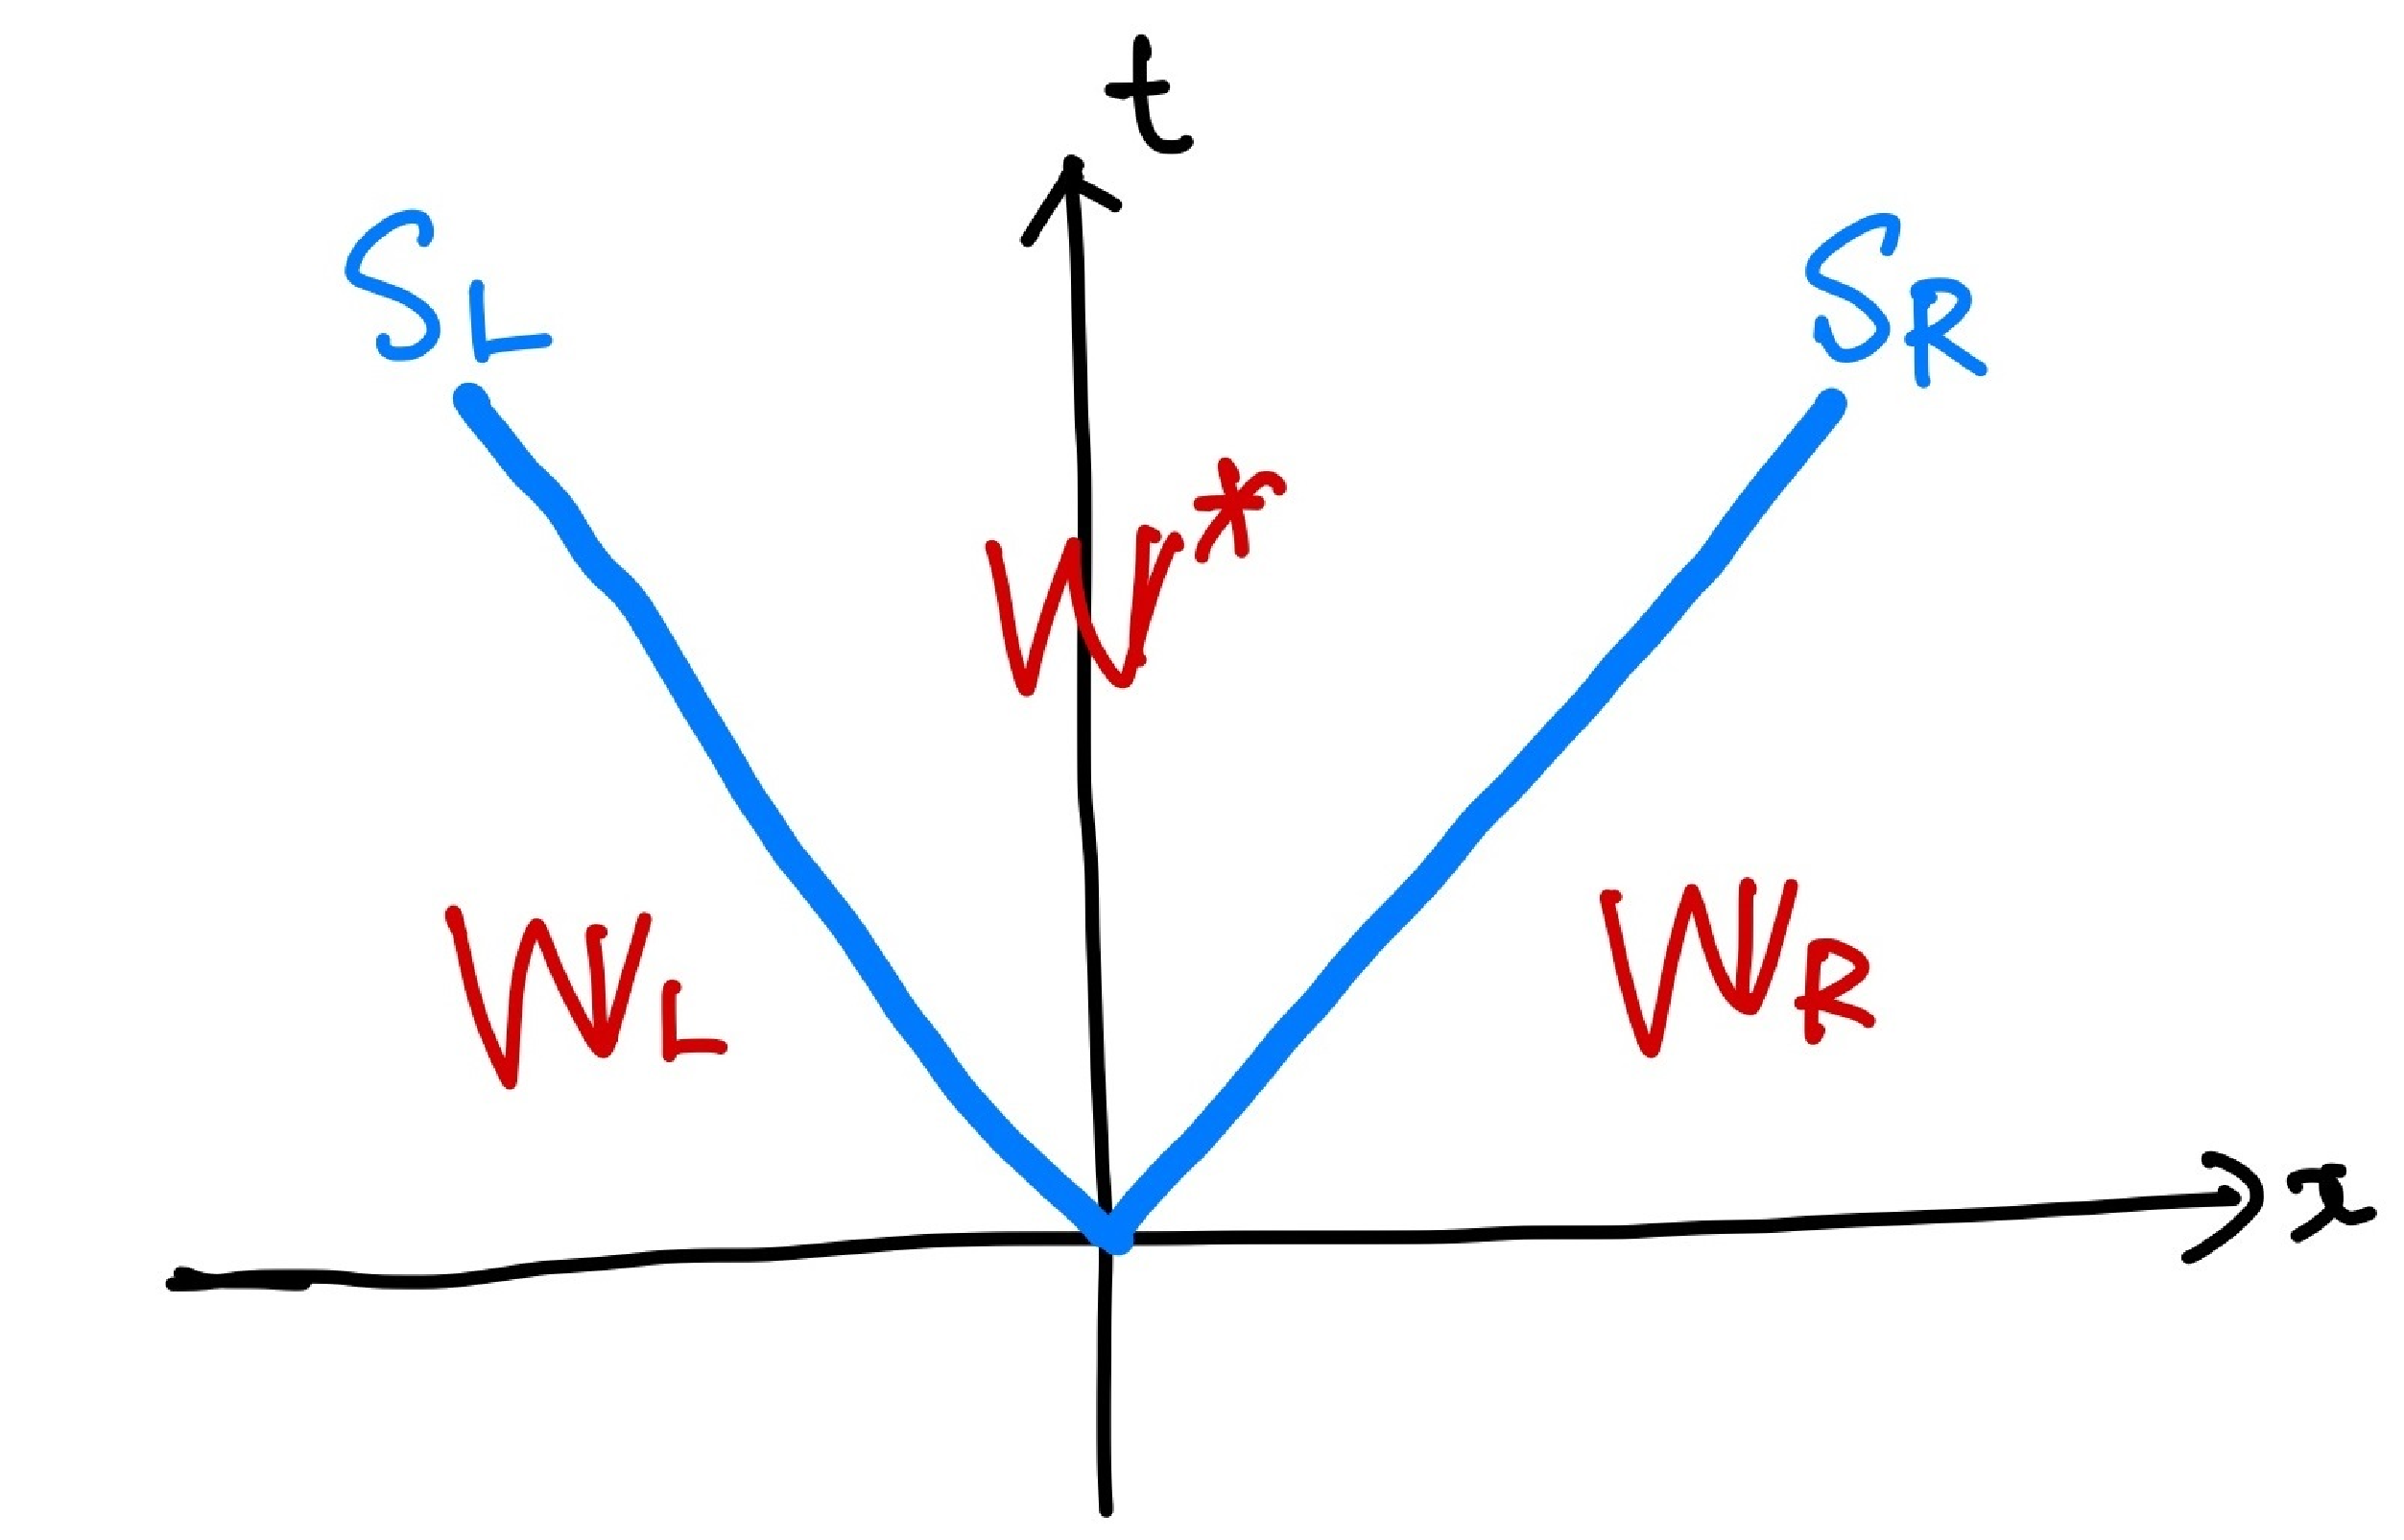
\includegraphics[width=10cm]{figures/HLL.pdf}
    \caption{
    HLL法
    }
    \label{fig:HLL}
\end{figure}

上記の場合分けの3つ目の場合は、中間状態の数値流束$\bm{ F}^*$が必要であるため、
以下で、その導出過程を示す。
HLL法では以下の保存式のみを使って中間状態を求める。
\begin{equation}
    \frac{\partial \bm{ U}}{\partial t}
    + \frac{\partial \bm{ F}}{\partial x} = \bm{ 0}
\end{equation}

まず、保存則を$\SL\Delta t\le x \le \SR\Delta t$と $0\le t\le \Delta t$で積分する。
\begin{equation}
    \int_{\SL\Delta t}^{\SR \Delta t} \bm{ U}(\Delta t, x) dx 
    - \int_{\SL\Delta t}^{\SR \Delta t}\bm{ U}(0, x)dx
    + \int_{0}^{\Delta t} \bm{ F}(t,\SR\Delta t) dt
    - \int_{0}^{\Delta t} \bm{ F}(t, \SL \Delta t) dt  = 0
\end{equation}
第一項は、時刻$t=\Delta t$で、$\SL\Delta t\le x \le \SR\Delta t$にある状態なので、
$\bm{ U}^* (\SR - \SL)\Delta t$となり、
第二項は、時刻$t=0$なので、$\SL\Delta t\le x\le 0$と$0\Delta t\le x\le \SR \Delta t$に
分割し、$\bm{ U}_\mathrm{L}\SL - \bm{ U}_\mathrm{R} \SR$となる。
第三項は、$x=\SR \Delta t$における$0\le t\le \Delta t$での状態なので、
$\bm{ F}_\mathrm{R}\Delta t$となり、第四項は、同様にして$-\bm{ F}_\mathrm{L}\Delta t$となる。
したがって、
\begin{equation}
\bm{ U}^* = \frac{
\SR \bm{ U}_\mathrm{R}
- \SL \bm{ U}_\mathrm{L}
- \bm{ F}_\mathrm{R} + \bm{ F}_\mathrm{L}
}{\SR - \SL}
\label{Ust_hll}
\end{equation}
を得る。

保存則を$0\le x\le \SR\Delta t$と $0\le t\le \Delta t$で積分すると、
\begin{equation}
    \int_0^{\SR\Delta t} \bm{ U}(\Delta t, x) dx 
    - \int_0^{\SR\Delta t}\bm{ U}(0, x)dx
    + \int_{0}^{\Delta t} \bm{ F}(t,\SR\Delta t) dt
    - \int_{0}^{\Delta t} \bm{ F}(t,0) dt  = 0
    \label{Fst_hll0}
\end{equation}
となり、図\ref{fig:HLL}より、
\begin{equation}
\bm{ U}_\mathrm{R} \SR \Delta t - \bm{ U}^* \SR \Delta t  
+ \bm{ F}_\mathrm{R}\Delta t - \bm{ F}^* \Delta t= 0
\end{equation}
を得る。
式(\ref{Ust_hll})を使うと、式(\ref{Fst_hll0})から、
\begin{screen}
\begin{equation}
\bm{ F}^* = \frac{
\SR \bm{ F}_\mathrm{L}
- \SL \bm{ R}_\mathrm{R}
+ \SR \SL \left(\bm{ U}_\mathrm{R} - \bm{ U}_\mathrm{L}\right)
}{\SR - \SL}
    \label{Fst_hll}
\end{equation}
\end{screen}
を得る。

\begin{screen}
HLL流束は
\begin{equation}
    \bm{ F}_\mathrm{HLL}
    =\left\{
    \begin{array}{ll}
         \bm{ F}_\mathrm{L} & \mathrm{if~\SL > 0} \\
         \bm{ F}_\mathrm{R} & \mathrm{if~\SR < 0} \\
         \bm{ F}^* & \mathrm{otherwise} \\
    \end{array}
    \right.
\end{equation}
\end{screen}

\vspace{1cm}

HLL法では、$\SL$と$\SR$は決まらないので、手で与える必要がある。
様々な手法が提案されている。
\begin{equation}
   \SL = \min(v_{x,\mathrm{L}}, v_{x,\mathrm{R}}) -  
    \max(c_\mathrm{s,L}, c_\mathrm{s,R}) ,\;\;\;
   \SR = \max(v_{x,\mathrm{L}}, v_{x,\mathrm{R}}) +  
    \max(c_\mathrm{s,L}, c_\mathrm{s,R}) 
\end{equation}

%--------------------------------------------------------
\clearpage
\subsubsection{HLLC近似Riemann解法}
%--------------------------------------------------------

HLLC(HLL-contact discontinuity)法は、HLL法の拡張である\citep{Toro1994}。
HLL法の中間状態を接触不連続面を介して、2つの状態($\bm{ U}_\mathrm{L}^*,\bm{ U}_\mathrm{R}^*$)
に分ける。

左右に伝播する波の前後での保存則より、
\begin{equation}
    \SL \bm{U}^*_\mathrm{L} - \bm{F}^*_\mathrm{L}
    = \SL \bm{U}_\mathrm{L} - \bm{F}_\mathrm{L}
    \label{hllc_sl}
\end{equation}
\begin{equation}
    \SR \bm{ U}_\mathrm{R}^* - \bm{ F}_\mathrm{R}^*
    = \SR \bm{ U}_\mathrm{R} - \bm{ F}_\mathrm{R}
    \label{hllc_sr}
\end{equation}
を得る。

接触不連続面なので、前後で速度と圧力が等しい。これらを$v^*$と$P^*$とする。
上の2つの保存式(式\ref{hllc_sl}、\ref{hllc_sr})の質量保存から、
\begin{equation}
 \rho_\mathrm{L}^* (\SL - v^*) = \rho_\mathrm{L} (\SL - v_\mathrm{L}) = C_\mathrm{L},\;\;\;
 \rho_\mathrm{R}^* (\SR - v^*) = \rho_\mathrm{R} (\SR - v_\mathrm{R}) = C_\mathrm{R}
 \label{hllc_mass}
\end{equation}
を得る。ここで、$C_\mathrm{L}$と$C_\mathrm{R}$は左右の波を介した質量流束を表す。

次に上の2つの保存式(式\ref{hllc_sl}、\ref{hllc_sr})の運動量保存から、
\begin{equation}
   - P^* + \rho_\mathrm{L}^* v^* (\SL - v^*) = 
   - P_\mathrm{L} + \rho_\mathrm{L} v_\mathrm{L}(\SL - v_\mathrm{L}),\;\;\;
   - P^* + \rho_\mathrm{R}^* v^* (\SR - v^*) = 
   - P_\mathrm{R} + \rho_\mathrm{R} v_\mathrm{R}(\SR - v_\mathrm{R}),\;\;\;
 \label{hllc_mom}
\end{equation}
となる。式(\ref{hllc_mass})を使うと、
\begin{equation}
   - P^* + C_\mathrm{L} v^* = 
   - P_\mathrm{L} + C_\mathrm{L} v_\mathrm{L},\;\;\;
   - P^* + C_\mathrm{R} v^* = 
   - P_\mathrm{R} + C_\mathrm{R} v_\mathrm{R}
 \label{hllc_mom}
\end{equation}
となり、$v^*$と$P^*$について解くと、
\begin{screen}
\begin{equation}
    v^* = \frac{ - C_\mathrm{L} v_\mathrm{L} + C_\mathrm{R} v_\mathrm{R} - (P_\mathrm{R} - P_\mathrm{L})}{-C_\mathrm{L} + C_\mathrm{R}} 
\end{equation}
\begin{equation}
    P^* = P_\mathrm{L} + C_\mathrm{L} (v^* - v_\mathrm{L})
        = P_\mathrm{R} + C_\mathrm{R} (v^* - v_\mathrm{R})
\end{equation}
\end{screen}
となる。これにより接触不連続面の伝播速度$S_\mathrm{M}=v_*$が決まる。

HLL方法と同じ考え方を使うと、$S_\mathrm{L}< S_\mathrm{M}<\SR$の3つの速度の正負で、
セル境界にある状態には4つの場合がありえる。したがって数値流束は以下で与えられる。
\begin{screen}
\begin{equation}
      \bm{ F}_\mathrm{HLLC} = \left\{
          \begin{array}{ll}
             \bm{ F}_\mathrm{L} & \mathrm{for~S_\mathrm{L}>0}\\
             \bm{ F}_\mathrm{L}^* = \bm{ F}_\mathrm{L} + S_\mathrm{L}\left( \bm{ U}_\mathrm{L}^* - \bm{ U}_\mathrm{L} \right)& \mathrm{for~S_\mathrm{L}\le 0 \le S_\mathrm{M}}\\
             \bm{ F}_\mathrm{R}^* = \bm{ F}_\mathrm{R} + S_\mathrm{R}\left( \bm{ U}_\mathrm{R}^* - \bm{ U}_\mathrm{R} \right)& \mathrm{for~S_\mathrm{M}\le 0 \le S_\mathrm{R}}\\
             \bm{ F}_\mathrm{R} & \mathrm{for~S_\mathrm{R}<0}\\
          \end{array}
      \right.
\end{equation}
\end{screen}
$\bm{ F}_\mathrm{L}^*$
と$\bm{ F}_\mathrm{R}^*$を求めるために、$\bm{ U}_\mathrm{L,R}^*$が必要である。
ここで重要なのは保存則だけを使うことである。

質量保存の式より、
\begin{equation}
     \rho_\mathrm{L,R}^* = \rho_\mathrm{L,R} 
     \frac{S_\mathrm{L,R} - u_\mathrm{L,R}}{ S_\mathrm{L,R} - S_\mathrm{M}}
\end{equation}
を得て、エネルギー保存式より、
\begin{equation}
  E_\mathrm{L,R}^* = \frac{ \left(S_\mathrm{L,R} - u_\mathrm{L,R}\right) E_\mathrm{L,R}
  - P_\mathrm{L,R}v_\mathrm{L,R} + P^* S_\mathrm{M}
  }{ S_\mathrm{L,R} - S_\mathrm{M}}
\end{equation}
を得る。中間状態$(\rho_\mathrm{L,R}^*,v^*, P^*, E_\mathrm{L,R}^*)$を使って、
$\bm{ F}_\mathrm{L,R}^*$を求める。

厳密Riemann解法ではないので、
HLL系解法では流体変数間の関係は満たされない。例えば、
\begin{equation}
    E_\mathrm{L,R}^* \ne \frac{1}{2}\rho_\mathrm{L,R}^* (v^*)^2 + P^*
\end{equation}
となるので注意。厳密解法ではもちろん一致する。




%\citep{Einfeldt1991}


%--------------------
\clearpage
\subsection{プログラミングするための準備}
%--------------------
Fortranを使ってプログラミングをおこなうための準備
をする。$x_i$や$\rho_i$、$F_{i+1/2}$など、空間に依存する量は
セルの番号をインデックスとする配列を使って表現する。
注意するのは、有限体積法ではセル中心で定義されている物理量($\rho_i$, $P_i$など)
とセル境界で定義されている物理量($F_{i+1/2}$)があることである。
Fortranでは、配列のインデックスは整数でなければならないので、
数値流束$F_{i+1/2}$の半整数{\ttfamily i+1/2}をインデックスにできない。
たとえば、数値流束$F_{i+1/2}$を{\ttfamily F(i)}と表現することにして、
頭の中で1/2だけずらす必要がある。

%--------------------
\subsubsection{座標に関する変数と配列}
%--------------------

図\ref{fig:hydro_mesh}に示す通り、
計算領域を$x_\mathrm{min}\le x\le x_\mathrm{max}$とし
(変数名 {\ttfamily x\_min}、{\ttfamily x\_max}),
空間を$N_\mathrm{grid}$個(変数名 {\ttfamily ngrid})のセルに分割する。

\ref{sec:ghost}節で述べた通り、境界条件を課すために使うゴーストセルを
左右に用意する(図\ref{fig:hydro_mesh}の赤破線)。
ゴーストセルの数は、Riemann問題の左右の状態を求める手法に依存する。
例えば、空間2次精度MUSCL法では、ゴーストセルは計算領域を挟み左右にそれぞれ2つ必要である。
ゴーストセルの数を、自由に変更できるようにするため、{\ttfamily mgn}という変数にする。

図\ref{fig:hydro_mesh}に示すように、
セル中心境界$x_{i-1/2}$を表す配列を{\ttfamily x1f(i)}とし、
セル中心座標を表す配列$x_i$を{\ttfamily x1v(i)}とする。
実はfortranでは配列の開始インデックスは任意の整数から始められるが、ここでは
デフォルトの1とする(C言語の場合0)。
ゴーストセルが加わるため、計算領域左端のセル中心座標のインデックスは1ではない値となり、
これを{\ttfamily is}とする(これは{\ttfamily mgn+1}と等しい)。
同様に右端のセル中心座標のインデックスを{\ttfamily ie}とする(これは{\ttfamily ngrid+mgn}と等しい)。
セル境界座標の{\ttfamily x1f(is)}は$x_\mathrm{min}$と等しく、
{\ttfamily x1f(ie+1)}は$x_\mathrm{max}$に等しい。

セル中心座標{\ttfamily x1f}の総要素数は{\ttfamily ngrid+2*ngh}で、
セル境界座標{\ttfamily x1v}の総要素数は{\ttfamily ngrid+2*ngh+1}である。
サンプルプログラムでは大きい方{\ttfamily ngrid+2*mgh+1}を
{\ttfamily in}としている。

\begin{figure}[htpb]
    \centering
    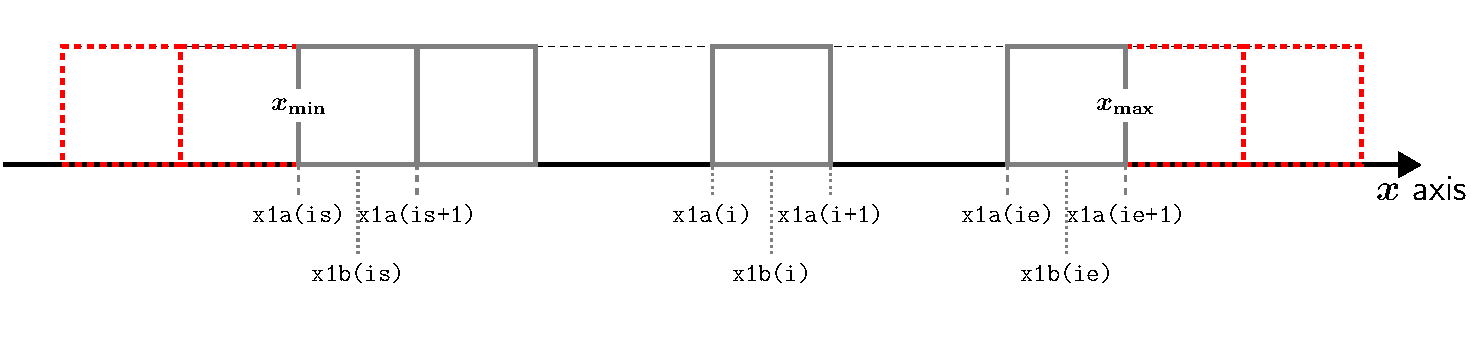
\includegraphics[width=17cm]{figures/hydro_mesh.pdf}
    \caption{
    }
    \label{fig:hydro_mesh}
\end{figure}

\begin{table}[h]
\begin{center}
\caption{座標に関する変数}
\begin{tabular}{|c|c|}
    \hline
    変数名/配列名 & 説明 \\
    \hline
    \hline
    {\ttfamily nx} & 計算領域内のセル総数 \\
    \hline
    {\ttfamily ngh} & ghost cell数 \\
    \hline
    {\ttfamily nxtot} & ghost cellを含めたセル総数 \\
    \hline
    {\ttfamily is} & 計算領域左端のセル番号\\
    \hline
    {\ttfamily ie} & 計算領域右端のセル番号\\
    \hline
    {\ttfamily x1min} & 計算領域左端の座標 \\
    \hline
    {\ttfamily x1max} & 計算領域右端の座標 \\
    \hline
    {\ttfamily x1c(i)} & セル中心の座標 $x_{i}$ (要素数 {\ttfamily nxtot}) \\
    \hline
    {\ttfamily x1b(i)} & セル境界の座標 $x_{i+1/2}$ (要素数 {\ttfamily nxtot+1}) \\
    \hline
\end{tabular}
\end{center}
\end{table}

%--------------------
\subsubsection{流体変数に関する変数と配列}
%--------------------
物理量は、$x$と$t$の2つの従属変数をもつので、
空間方向のセル番号と時間ステップの番号を引数とする
2次元配列、例えば{\ttfamily d(i,n)}で定義するのが自然と思うかもしれない。
しかし、例えばオイラー時間積分法で解く場合、$t=t^{n+1}$での$U$を求めるとき、
前の時刻$t=t^n$の全空間の$U$のデータを保存しておけば十分で、
それ以前$t\le t^{n-1}$のデータは不要である。
したがって、通常、時間ステップ番号を引数とすることはなく、
空間1次元のシミュレーションをおこなう場合は、
セル番号を引数とする配列(例えば{\ttfamily U(i)})を宣言する。
多段の時間積分法を使う場合は、サブステップの物理量を保存しておく必要があるため、
必要な数の配列を宣言する。

\vspace{1cm}

サンプルコードでは、保存量と基本量をそれぞれ2次元配列{\ttfamily U(i,n)}と{\ttfamily W(i,n)}
で定義している。一番目の引数{\ttfamily i}はセル番号を表し、二番目の引数{\ttfamily n}は
流体変数のインデックスを表す。
1次元流体計算では式(\ref{hydro1d_eq})で示すように、3つの要素をもつ。
たとえば、{\ttfamily U(i,0)}は、i番目のセルの密度を表し、
{\ttfamily W(i,2)}はi番目のセルの圧力を表す。
プログラム内で、番号で流体変数の種類を指定するのは間違いの元なので、
変数名を流体変数と対応付けた整数変数を定義する。詳しくは表\ref{tab:phys}を参照。



%有限体積法であるため、
%時間ステップの更新は保存量$\rho, m, E$でおこなう。
%基本量$\rho, v, P$は保存量から導出できるので、保存量さえ
%配列として保持しておけば事足りる。
%しかし、基本量もプログラム内でよく使う
%(例えばMUSCL法で内挿する物理量としてよく使われる)ので、
%基本量も配列として保持する。
%その他、内部エネルギーと音速も保持する。
%セル境界で定義される数値流束を質量と運動量・エネルギー保存方程式の3つ保持する。

表\ref{tab:phys}にサンプルプログラムで使われている配列を示す。




\begin{table}[h]
\begin{center}
\caption{流体変数に関する変数}
\begin{tabular}{|c|c|}
    \hline
    変数名/配列名 & 説明 \\
    \hline
    \hline
    \multicolumn{2}{|l|}{ {\bf 基本量} (primitive variables){\ttfamily (IDEN=0, IVX=1, IPRE=2)}} \\
    \hline
    {\ttfamily Q(i,IDN)} & $x=x_i$における密度 (要素数 {\ttfamily nxtot}),   \\
    \hline
    {\ttfamily Q(i,IV1)} & $x=x_i$における速度 (要素数 {\ttfamily nxtot}) \\
    \hline
    {\ttfamily Q(i,IPR)} & $x=x_i$における圧力 (要素数 {\ttfamily nxtot}) \\
    \hline
    \multicolumn{2}{|l|}{ {\bf 保存量} (primitive variables) {\ttfamily (IDEN=0, IMX=1, IENE=2)}} \\
    \hline
    {\ttfamily U(i,IDN)} & $x=x_i$における密度 (要素数 {\ttfamily nxtot}) \\
    \hline
    {\ttfamily U(i,IM1)} & $x=x_i$における運動量 (要素数 {\ttfamily nxtot}) \\
    \hline
    {\ttfamily U(i,IEN)} & $x=x_i$における全エネルギー (要素数 {\ttfamily nxtot}) \\
    \hline
    \multicolumn{2}{|l|}{ {\bf セル境界の流束} (numerical flux) {\ttfamily (IDEN=0, IMX=1, IENE=2)}} \\
    \hline
    {\ttfamily F(i,IDN)} & $x=x_{i+1/2}$における質量流束 (要素数 {\ttfamily nxtot+1}) \\
    \hline
    {\ttfamily F(i,IM1)} & $x=x_{i+1/2}$における運動量流束 (要素数 {\ttfamily nxtot+1}) \\
    \hline
    {\ttfamily F(i,IEN)} & $x=x_{i+1/2}$におけるエネルギー流束 (要素数 {\ttfamily nxtot+1}) \\
    \hline
\end{tabular}
\end{center}
\label{tab:phys}
\end{table}



%--------------------
\subsection{ゴーストセルを使った境界条件の処理}
%--------------------

流体方程式は、偏微分方程式なので解くためには境界条件が必要となる。
時間方向の境界条件は初期条件と呼ばれ、シミュレーション上では、$t=0$において、
全てのセルの$U$に値を代入することに対応する。

現実の空間は無限に広がっているが、シミュレーションをおこなう場合は、有限の計算領域を
設定せざるを得ず、必ず空間方向の境界条件(以下では単に境界条件と呼ぶ)を
与える必要がある。

代表的な境界条件としては、
\begin{itemize}
    \item 周期境界条件 $U(x+L) = U(x)$

    \item ディリクレ境界条件 $\partial U/\partial x=U_0'$.

    \item ノイマン境界条件 $U=U_0$
\end{itemize}
がある。その他、問題設定に応じて適切な条件を設定する。

左端セルの密度の時間発展は、
\begin{screen}
{\ttfamily
\small
  U(is,IDEN) = U(is,IDEN) - dt/(x1f(is+1) - x1f(is))*( F(is+1,IDEN) - F(is,IDEN) )
}
\end{screen}
となる。ここで{\ttfamily F(is,IDEN)}は{\ttfamily U(is-1,IDEN)}と{\ttfamily U(is,IDEN)}
から計算されるはずだが、
{\ttfamily U(is-1,IDEN)}は計算領域外にあるので、このままでは{\ttfamily F(is,IDEN)}が計算できない。
計算領域の右端のセルも同様に時間発展できない。

境界条件を設定する方法は色々ある。
たとえば、計算領域の境界における数値流束{\ttfamily F(IDEN,is)}を、
境界条件を満たすように直接与えるのも一つの手である。
流束が0の境界条件であれば、{\ttfamily dflux(is)=0}にすればよい。
ただその場合は、境界のセルを特別扱いする必要がある。

昨今の公開コードで多く用いられているのは、計算領域の外に「ゴースト」セルを用意する方法である。
設定したい境界条件が満たされるようにゴーストセルに値を事前に代入すれば、
計算領域の境界と接しているセルも、そうでないセルと全く同じ手順で計算できるため、コードが簡潔になる。

\begin{itemize}
    \item 周期境界条件の場合$U(x+L)=U(x)$

        {\ttfamily x1v(is-1)}と{\ttfamily x1v(ie)}が同一視される。また、
        {\ttfamily x1v(ie+1)}と{\ttfamily x1v(is)}が同一視される。

        したがって、ゴーストセルに代入すべき値は、
        \begin{screen}
                {\ttfamily U(is-1,IDN) = U(ie,IDN)} \\
                {\ttfamily U(ie+1,IDN) = U(is,IDN)}
        \end{screen}

    \item ディレクレ条件の場合 $\partial U/\partial x =U_0'$

        左端に着目すると、計算領域の右端の境界{\ttfamily xf(is)}での$U$の勾配を差分化すると、
        \begin{equation}
            \frac{U_{is} - U_{is-1}}{\Delta x} = U_0'
        \end{equation}
    となる。したがって、$U_{is-1} = U_{is} - U_0' \Delta x$となる。
    同様に、左端の境界{\ttfamily xf(ie+1)}では、
    $U_{ie+1} = U_{ie} + U_0' \Delta x$が得られる。

    \item ノイマン条件の場合 $U=U_0$

        物理量がセル中心でしか定義されていないので、ゴーストセルの値を使って、セル境界の値を最も簡単に表すと、
        $U(x_{is})= (U_{is} + U_{is-1})/2$となる。
        これが$U_0$に等しいので、$U_{is-1} = 2U_0 - U_{is}$が得られる($U_0$と$U_{is-1}$を使った外挿になっている)。
        右端の境界でも同様にして、$U_{ie+1} = 2U_0 - U_{ie}$を得る。

\end{itemize}

%--------------------
\subsection{時間空間一次精度サンプルプログラムでの計算手順}
%--------------------

%図\ref{fig:fc_HD1}に、サンプルプログラムの計算手順を示す。
以下にサンプルプログラムの計算手順を示す(図\ref{fig:fc_HD1}のフローチャットも参照)。
対応する関数およびサブルーチンを載せている。

引数に色を付けている。赤がインプットに対応する変数/配列(サブルーチン内で変更しない)で、
青がサブルーチン内で値を代入する変数/配列を表す。

\begin{enumerate} 
     \item シミュレーションを始める前の準備
     \begin{itemize}
        \item まず、セル境界とセル中心の座標の設定をする。
        \begin{itemize}
            \item {\ttfamily GenerateGrid( {{\color{red}xf, xv} })} 
        \end{itemize}
        \item 基本量の初期分布を設定する。
        \begin{itemize}
            \item {\ttfamily GenerateProblem( {\color{blue} x1c, x1b}, {\color{red} W} )}
        \end{itemize}
        \item 保存量に変換
        \begin{itemize}
            \item {\ttfamily ConsvVariable( {\color{blue} Q}, {\color{red} U} )}
        \end{itemize}
     \end{itemize}

     \item シミュレーションのメインループ (ここで物理量の時間を更新する)
     \begin{itemize}
         \item CFL条件を満たすように$\Delta t$を設定する。 
         \begin{itemize}
             \item  {\ttfamily Real(8) Function 
             TimeControl( {\color{blue}x1a, Q} )}
         \end{itemize}
         \item 境界条件を設定するためにゴーストセルに適切な値を代入する。
         \begin{itemize}
             \item  {\ttfamily BoundaryCondition( {\color{red} Q} )}
           \end{itemize}
           \item 数値流束を求める。 
           \begin{itemize}
               \item  {\ttfamily NumericalFlux( {\color{blue} x1a, xv, Q}, {\color{red} F} )}
           \end{itemize}
          \item 保存量を更新する。 
          \begin{itemize}
              \item  {\ttfamily UpdateConsv( {\color{blue} dt, xf, Uold, F}, {\color{red} U} )}
          \end{itemize}
            
          
          \item 保存量から基本量を求める。
          \begin{itemize}
              \item  {\ttfamily PrimVariable( {\color{blue} U}, {\color{red} Q} )}
          \end{itemize}
          

          \item 必要なら結果を出力する。
          \begin{itemize}
              \item {\ttfamily Output( {\color{blue} x1a, x1b, U, Q} )}
          \end{itemize}
          
          \item 時間を更新し ({\ttfamily time = time + dt})、シミュレーションの終了条件を満たしているか確認し、満たしていたらメインループを抜ける。満たしていなかったら、メインループの始めに戻る。
          
     \end{itemize}
\end{enumerate}


\begin{figure}[h]
    \centering
    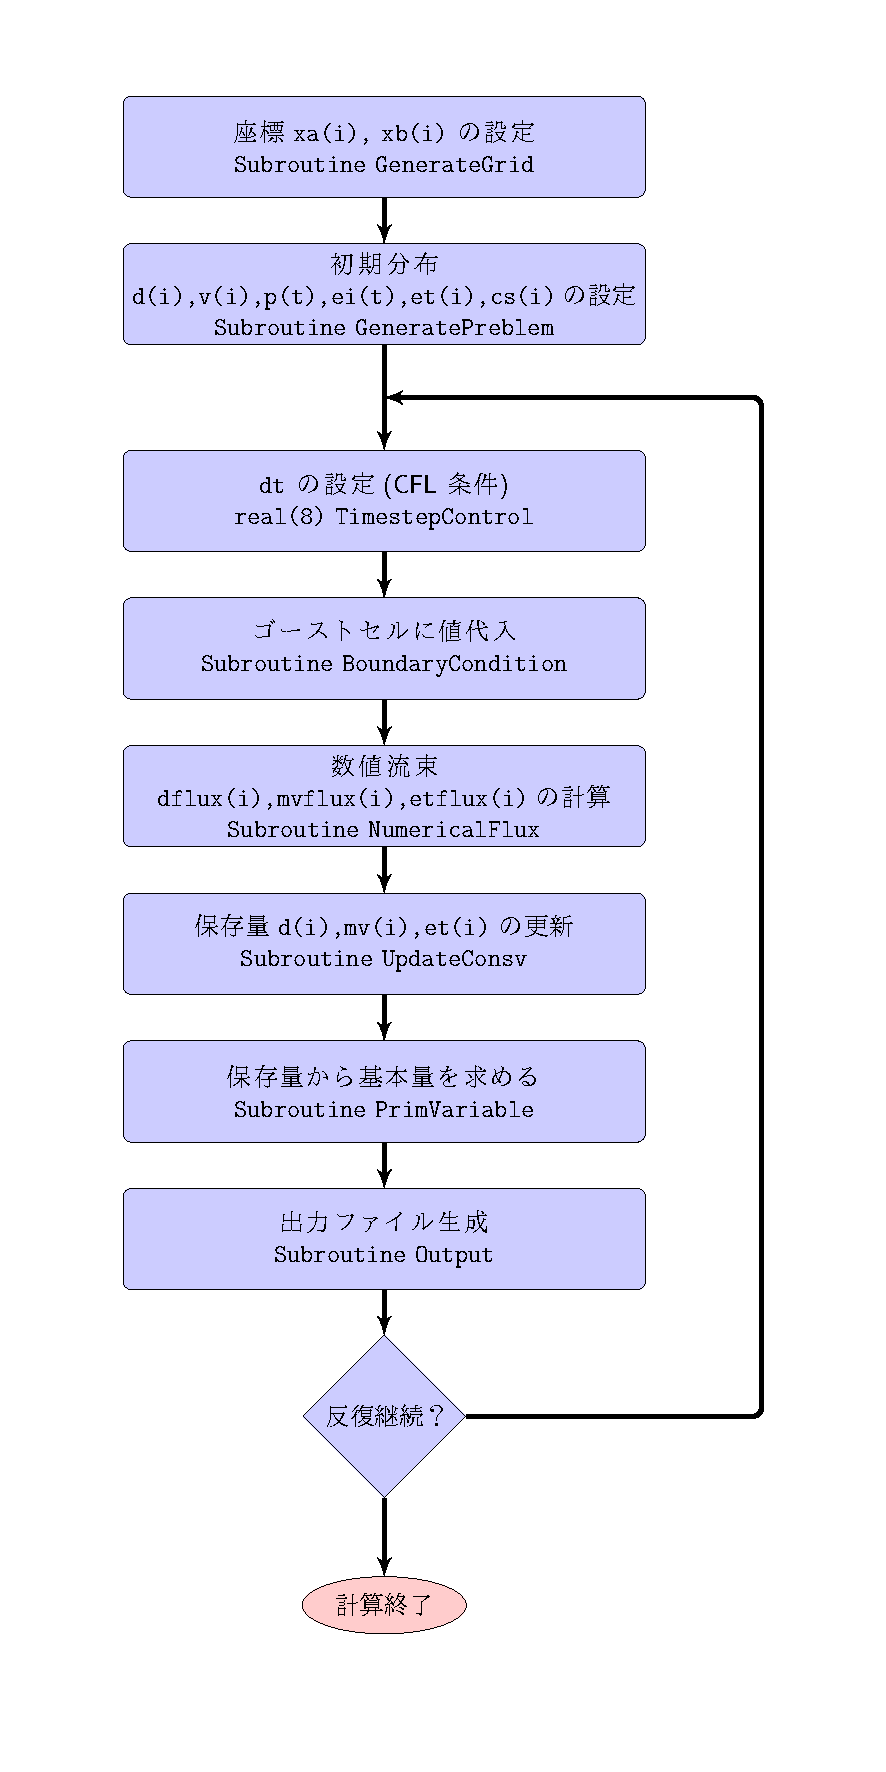
\includegraphics[width=5cm]{figures/flowchart_HD1.pdf}
    \caption{サンプルプログラムの計算手順のフローチャート。
    }
    \label{fig:fc_HD1}
\end{figure}


\subsubsection{サンプルコードで使わている変数の説明}

\begin{table}[h]
\begin{center}
\caption{時間発展に関数する変数}
\begin{tabular}{|c|c|}
    \hline
    変数名/配列名 & 説明 \\
    \hline
    \hline
    {\ttfamily nhy} & 時間ステップ数 \\
    \hline
    {\ttfamily nhymax} & 最大時間ステップ数 \\
    \hline
    {\ttfamily time } & 時刻 \\
    \hline
    {\ttfamily timemax } & 計算終了時刻 \\
    \hline
    {\ttfamily dt} & 時間幅 \\
    \hline
\end{tabular}
\end{center}
\caption{ {\ttfamily nhy $>$ nhymax}または{\ttfamily time $>$ timemax}を満たすと計算が終了する。}
\end{table}

%======================================================================
\clearpage
\section{実習課題}
%======================================================================

%--------------------------------------------------
\subsection{衝撃波管問題}
%--------------------------------------------------
まずは問題設定が単純な衝撃波管問題でコードが正しく動いてるかを確認する。

\subsubsection{理論}

詳しくは講義資料を参照のこと。
不連続面で仕切られた2つの一様なガスの時間進化には、厳密解が知られており、
数値流体計算コードが正しく動いているかをテストするためによく使われる。
%Godunov法では、各セル境界でRiemann問題を解いて数値流束を求めている。

Sod解は有名な衝撃波管問題の解で、計算コードの論文によく登場する。
左右の物理量を添え字"L"と"R"を使ってそれぞれ表すと、
Sod解の初期条件は、
\begin{equation}
\left(
\begin{array}{c}
\rho_\mathrm{L} \\
v_\mathrm{L} \\
P_\mathrm{L} \\
\end{array}
\right)
= 
\left(
\begin{array}{c}
1 \\
0 \\
1 \\
\end{array}
\right),\;\;\;
\left(
\begin{array}{c}
\rho_\mathrm{R} \\
v_\mathrm{R} \\
P_\mathrm{R} \\
\end{array}
\right)
= 
\left(
\begin{array}{c}
0.125 \\
0 \\
0.1 \\
\end{array}
\right)
\end{equation}
である。
伝統的にSod解での比熱比は$\gamma=1.4$が使われる。

計算結果と比較するための解析解を生成する{\ttfamily python}スクリプト({\ttfamily RiemannSolver.py})を用意した。
すでに生成したファイル{\ttfamily sod\_ana.dat}(時刻$t=0.2$での解析解。
1列目は$x$、2列目は$\rho$、3列目は$v$、4列目は$P$。)をディレクトリの中に入れている。
 
図\ref{fig:sodana}は$t=0.2$における厳密解を表す。
左のガスの方が高圧なので、右のガスから左のガスが押されて、
右のガスに衝撃波が伝わり、逆に右のガスには希薄波が生じる。

\begin{figure}[htpb]
    \centering
    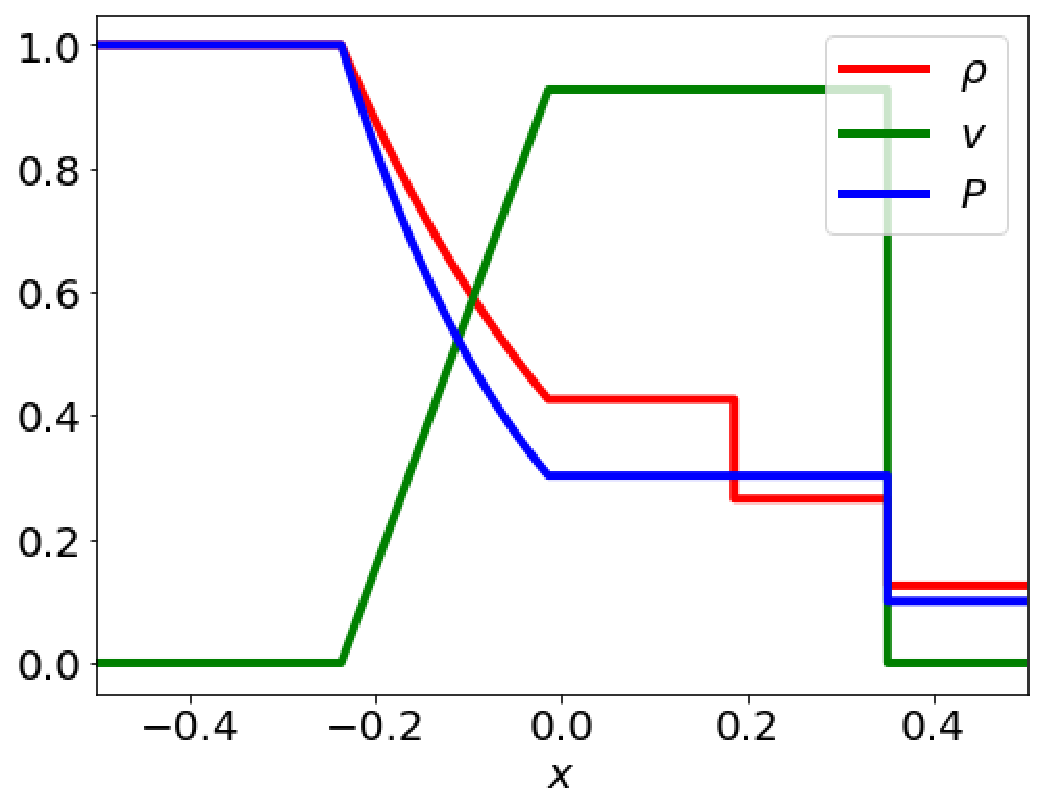
\includegraphics[width=8cm]{figures/sod.pdf}
    \caption{$t=0.2$におけるSod解}
    \label{fig:sodana}
\end{figure}





\subsubsection{出力}

サンプルコードでは、{\ttfamily dtout}毎にスナップショットファイルの出力をおこなっている。
対応するサブルーチンは{\ttfamily Output}である。
スナップショットファイルは、ディレクトリ{\ttfamily snap/}の下に作られる。

\subsubsection{可視化}

可視化はシミュレーション結果を確認する強力な方法である。
この実習では計算コードを実装しつつ、衝撃波管問題の解析解と比較する。
参考のために{\ttfamily gnuplot}と{\ttfamily python}による可視化のためのサンプルコードを用意した。

\begin{itemize}
    \item  {\bf {\ttfamily gnuplot}によるインタラクティブな可視化} \\
    コマンドラインで{\ttfamily gnuplot}と入力
    すると起動する。

    \begin{screen}
    {\ttfamily gnuplot> plot "snap/t00001.dat" using 1:2}
    \end{screen}
  と入力すると横軸を1列目、縦軸を2列目にとったグラフが出力される。

    解析解と同時に出力したい場合は、
    \begin{screen}
    \small
    {\ttfamily gnuplot> plot "snap/t00001.dat" using 1:2 w lp, "sod\_ana.dat" using 1:2 w l}
    \end{screen}

    {\ttfamily using}の後の列を指定する箇所は、演算した結果を使うこともできる。\\
    たとえば、
    {\ttfamily using (\$1*2):(\$2*\$3)}にすると、1列目を2倍した値を横軸とし、
    2列目と3列目の積の値を縦軸にとったプロットを作れる。


    \item {\bf {\ttfamily gnuplot}によるパラパラ漫画出力}

    {\ttfamily gnuplot}の出力画面上で、パラパラ漫画のように各時刻のスナップショットを連続的に
    表示できる。
    コマンドラインで、
    \begin{screen}
    \small
    {\ttfamily gnuplot RealtimeAnime.plt}
    \end{screen}
    を実行する。
    {\ttfamily gnuplot}を起動した上で実行する場合は、{\ttfamily load "RealtimeAnime.plt"}を実行する。
    
    \item {\bf {\ttfamily gnuplot}による動画の作成}

    {\ttfamily MakeAnime.sh}は、
    {\ttfamily snap/}に出力されたファイルをつかって、自動で動画を作るスクリプトである。

    コマンドラインで、
    \begin{screen}
    \small
    {\ttfamily ./MakeAnime.sh}
    \end{screen}
    を実行すると、動画ファイル{\ttfamily animation.mp4}が作成される。再生する場合は、
    コマンドラインで
    \begin{screen}
    \small
    {\ttfamily mplayer animation.mp4}
    \end{screen}
    を実行する。
    
    
    \item {\bf {\ttfamily python}による動画の作成}

    コマンドラインで
    \begin{screen}
    \small
    {\ttfamily python MakeAnime.py}
    \end{screen}
    を実行する。
    
\end{itemize}


\subsubsection{課題}

サンプルプログラムに以下を実装し
\begin{itemize}
    \item 数値流束 HLL法 (HLL法を実装したあと余力があればHLLC法も)
    \item outflow境界条件の設定(すべての基本量の勾配を境界で0にする)
    {\ttfamily BoundaryCondition}
\end{itemize}
シミュレーション結果が厳密解と整合的か確認する。
特に接触不連続面の両側の物理量が厳密解と一致しているか。



%======================================================================
\newpage
\subsection{音波の伝播}
%======================================================================

%--------------------------------------------------
\subsubsection{理論}
%--------------------------------------------------

基礎方程式は以下になる。ここで便利のために全エネルギー保存の式を断熱の式に置き換えている。
\begin{equation}
    \frac{\partial \rho}{\partial t} + \frac{\partial \rho v}{\partial x} = 0
\end{equation}
\begin{equation}
    \rho\left(\frac{\partial v}{\partial t} + v\frac{\partial v}{\partial x}\right) =
    - \frac{\partial P}{\partial x} 
\end{equation}
\begin{equation}
   \left(\frac{\partial }{\partial t} + v\frac{\partial }{\partial x}\right)
   \ln \left(\frac{P}{\rho^\gamma}\right) = 0
\end{equation}
非摂動状態として一様な静止したガスを考える(密度$\rho=\rho_0$、速度$v=0$、圧力$P=P_0$)。
摂動量を$\delta \rho$, $\delta v$、$\delta P$とし、流体方程式を線形化すると,
\begin{equation}
    \frac{\partial \delta \rho}{\partial t} + \rho_0 \frac{\partial \delta v}{\partial x} = 0
    \label{eoc_sound}
\end{equation}
\begin{equation}
    \rho_0\frac{\partial \delta v}{\partial t} = 
    - \frac{\partial \delta P}{\partial x} 
    \label{eom_sound}
\end{equation}
\begin{equation}
\frac{\delta P}{P_0} -\gamma \frac{\delta \rho}{\rho_0}  = 0 \;\;\;
\Rightarrow \;\;\; \delta P = c_\mathrm{s}^2 \delta \rho,
    \label{eoe_sound}
\end{equation}
ここで、$c_\mathrm{s}=\sqrt{\gamma P_0/\rho_0}$は音速である。

式(\ref{eoe_sound})を式(\ref{eom_sound})に代入し、式(\ref{eoc_sound})を使って、
$\delta v$を消去すると、以下の$\delta \rho$についての波動方程式を得る。
\begin{equation}
    \frac{\partial \delta \rho}{\partial t^2} - c_\mathrm{s}^2 \frac{\partial \delta \rho}{\partial x^2}=0
\end{equation}
ちなみに$\delta v$と$\delta P$も全く同じ波動方程式に従う。
波動方程式の厳密解は、よく知られており、波形を保ったまま左右に伝播する波を
表す($\delta \rho(x,t) = g(x-ct) + f(x+ct)$)。

%---------------------------------------
\subsubsection{課題1}
%---------------------------------------

密度摂動が、
\begin{equation}
    \delta \rho(x,t) = A \sin ( k(x - c_\mathrm{s}t))
\end{equation}
に従って、右に伝わる様子をシミュレーションしよう。
ここで$k$は波数である。

密度摂動が上の式で与えられたとき、速度摂動と圧力摂動がどう与えられるかは、
摂動方程式からわかるので、適切な初期条件を与えること。


%一次元流体方程式を有限体積法を使って離散化すると,
%\begin{equation}
%    \bm{ U}_{i}^{n+1} = \bm{ U}_{i}^n 
%    - \frac{\Delta t}{\Delta x}\left( \bm{ F}_{i+1/2}^{n+1/2} - \bm{ F}_{i-1/2}^{n+1/2} \right)
%\end{equation}
%を得る。





